In this chapter, we will formalize measurement biases of magnetometers. First we give an overview, followed by a physical explanation. Then, we provide a model that includes major biases and introduce a desirable decomposition of the magnetic field. At the end, we summarize different approaches for magnetometer calibration which were developed in the past.

\section{Overview}

Measurement biases of magnetometers in smartphones are caused by magnetic materials inside the phone which interfere with the external magnetic field. The measurement bias is usually decomposed into two different effects: the hard iron and the soft iron effect. Figure \ref{fig:hard_soft_iron} is an example of how hard and soft iron effects influence the measurement of the magnetometer after a full rotation of the sensor along an arbitrary axis in a homogeneous magnetic field.

The hard iron effect of magnetometers in smartphones is due to magnetic materials inside the phone which retain their magnetism even after the removal of the external magnetic fields. A permanent magnet of the speaker inside the phone is an example for that. Since these components are firmly attached to the magnetometer, the hard iron effect will cause an offset between the external and the measured magnetic field. The magnetization of the materials in the phone can still change in strength and direction in presents of external fields which adds dynamics to the hard iron effect.

The soft iron effect is due to inhomogeneous magnetization of materials in the smartphone in presence of external magnetic fields. This effect distorts the measurement of the magnetometer depending upon which direction the field acts relative to the sensor. In contrast to the hard iron effect, the soft iron effect does not bias measurements in absence of external magnetic fields.

Usually, the hard iron effect has a much larger contribution to the total uncorrected error than soft iron effect.\cite{vectornav}

\begin{figure}[hbt!]
    \centering
    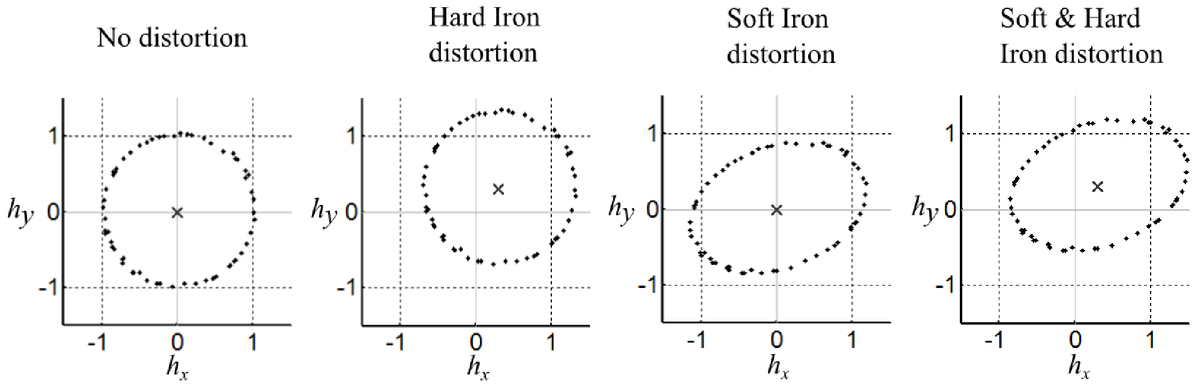
\includegraphics[width=0.8\textwidth]{figures/hard_soft_iron.jpg}
    \caption{Illustration of the hard and soft iron effect.\cite{hard_soft_iron}}
    \label{fig:hard_soft_iron}
\end{figure}

As discovered during working on this thesis, iOS and Android only provide magnetometer measurements without hard iron calibration but with soft iron and temperature calibration. This suggests that the soft iron effect and temperature dependencies are calibrated by the sensor hardware and the hard iron effect is calibrated by software of the \gls{os} or manufacturer. In this case the calibration depends on different algorithms across different devices. Treating their estimates equally is an additional source of error in cross-device scenarios, such as \gls{ips} (see Sections \ref{sec:ips} for more details). Moreover the operating system does not quantify the goodness of the hard iron calibration and requires unnatural movements of the phone to perform the calibration.

\section{Physical origin}
% http://hyperphysics.phy-astr.gsu.edu/hbase/Solids/hyst.html#c3
% http://hyperphysics.phy-astr.gsu.edu/hbase/Solids/ferro.html#c4
% TODO mention magnetic domains? https://en.wikipedia.org/wiki/Magnetic_domain

The soft and hard iron effects can be explained by magnetic hysteresis. It occurs when a ferromagnet, such as iron, is exposed to an external magnetic field and the magnetic dipoles of the atoms align with it. Some of the alignments will remain even after removing the external field which is called remanence. The material has become magnetized and will remain so indefinitely. In order to demagnetize it one has to apply heat or a sufficiently strong external magnetic field in the opposite direction.

Magnetic hysteresis can be visualized with a $\bm{H}$-$\bm{M}$ or $\bm{H}$-$\bm{B}$ diagram. An example is given in Figure \ref{fig:magnetic_hysteresis}. In general the relationship between the external magnetic field strength $\bm{H}$ and the magnetization $\bm{M}$ is not linear. The origin of the diagram ($\bm{H}=\bm{M}=\bm{0}$) denotes the demagnetized state of the material in absence of external fields. Increasing the external field $\bm{H}$ in one direction leads to an increasing magnetization $\bm{M}$ until saturation is reached. All dipoles point in the same direction. After removing the external field the material is still magnetized. This is called remanence and is denoted by $\bm{B}_r$ in the diagram. Reversing the external field will weaken the magnetization until it vanishes at $\bm{H}_c$, called coercivity.

Note that this is a one dimensional simplification of a more complicated three-dimensional situation.

\begin{figure}[hbt!]
    \centering
    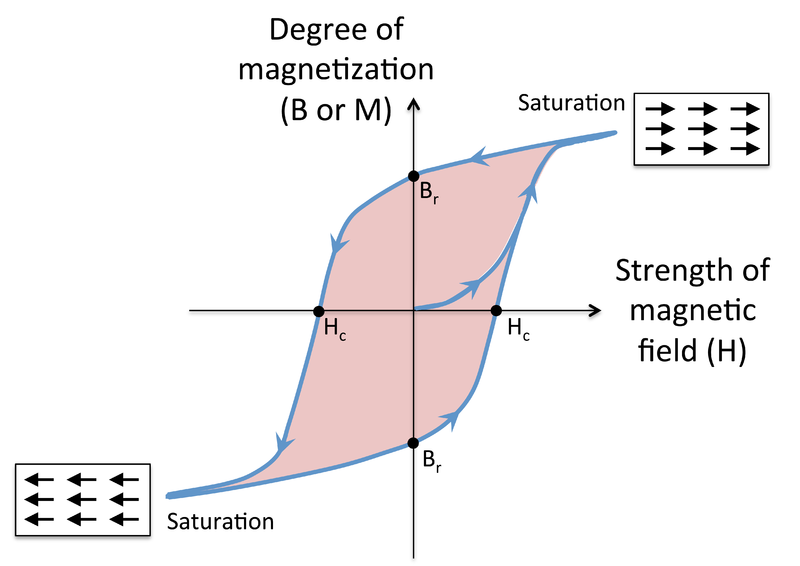
\includegraphics[width=0.8\textwidth]{figures/magnetic_hysteresis.png}
    \caption{Illustration of the magnetic hysteresis.}
    \label{fig:magnetic_hysteresis}
\end{figure}

Ferromagnetic materials can be divided into magnetically soft and hard materials. Soft materials can be magnetized but do not tend to stay so because of low coercivity. Hard materials tend to stay magnetized because of high coercivity and can be used as permanent magnets.

The soft iron effect is caused by magnetically soft materials which magnetize in the presents of external fields and therefore amplify it. In general this effect is anisotropic because of the geometry of the material and its relative position to the magnetometer.

The hard iron effect is caused by magnetically hard materials which remain magnetized in absence of external fields. Since the magnetometer is firmly attached to the magnetically hard materials, this effect will cause an offset of the measurement, independent of the orientation of the sensor. Because of the magnetic hysteresis, the hard iron offset will change over time in presence of sufficiently strong and altering external magnetic fields.

\section{Magnetometer sensor model}

Equation \ref{eq:magnetometer_model} is a model for magnetometer measurements that includes soft and hard iron effects. The soft iron effect is parameterized with 6 values ($s_x$, $s_y$, $s_z$, $s_{xy}$, $s_{xz}$, $s_{yz}$) which scale and shear the magnetic field $\bm{B}$. The hard iron effect is parameterized with 3 values ($h_x$, $h_y$, $h_z$) which shift the external magnetic field vector $\bm{B}$. $\bm{B}_\text{noise}$ is the measurement noise of the magnetometer, which could be modeled as zero-centered Gaussian noise.\cite{vectornav}

Equation \ref{eq:magnetometer_model_inv} is the inverse of \ref{eq:magnetometer_model} which can be used estimate the magnetic field $\bm{B}$ from a measurement $\bm{B}_\text{measure}$, given the soft and hard iron parameters.

\begin{equation}
\label{eq:magnetometer_model}
    \bm{B}_\text{measure} = \left[\begin{matrix}
    1 & s_{xy} & s_{xz}\\
    0 & 1 & s_{yz}\\
    0 & 0 & 1\\
    \end{matrix}\right] \times \left[\begin{matrix}
    s_x & 0 & 0\\
    0 & s_y & 0\\
    0 & 0 & s_z\end{matrix}\right] \times \left(\bm{B} + \left[\begin{matrix}h_x\\h_y\\h_z\end{matrix}\right]\right) + \bm{B}_\text{noise}
\end{equation}

\begin{equation}
\label{eq:magnetometer_model_inv}
    \hat{\bm{B}} = \left[\begin{matrix}
    \frac{1}{s_x} & 0 & 0\\
    0 & \frac{1}{s_y} & 0\\
    0 & 0 & \frac{1}{s_z}\end{matrix}\right] \times \left[\begin{matrix}
    1 & s_{xy}^* & s_{xz}^*\\
    0 & 1 & s_{yz}^*\\
    0 & 0 & 1\\
    \end{matrix}\right] \times \bm{B}_\text{measure} - \left[\begin{matrix}h_x\\h_y\\h_z\end{matrix}\right]
\end{equation}

In case of a misalignment between device and sensor axis an additional rotation is required with 3 parameters.

Temperature dependencies can be modeled with polynomials for each parameter.

\section{Decomposition}

Neglecting the soft iron effect, the measurement of the magnetometer can be expressed by the following decomposition.

\begin{equation}
\label{eq:decomposition}
    \bm{B}_\text{measure}(t, \bm{x}) = \bm{B}_\text{phone}(t) + \bm{B}(t, \bm{x}) + \bm{B}_\text{noise}
\end{equation}

\begin{equation}
\label{eq:decomposition_earth_env}
    \bm{B}(t, \bm{x}) = \bm{B}_\text{earth}(t, \bm{x}) + \bm{B}_\text{env}(t, \bm{x})
\end{equation}

Where $\bm{B}_\text{measure}(t, \bm{x})$ is the measurement of the magnetometer at a given point in time and space, $\bm{B}_\text{phone}(t)$ the magnetic field created by the smartphone, $\bm{B}(t, \bm{x})$ is the external magnetic field, $\bm{B}_\text{earth}(t, \bm{x})$ the magnetic field of the earth, $\bm{B}_\text{env}(t, \bm{x})$ is the magnetic field of the environment, and $\bm{B}_\text{noise}$ the noise produced by the magnetometer.

In pedestrian navigation, localization and wayfinding scenarios one can neglect the time dependency of $\bm{B}_\text{earth}$ and $\bm{B}_\text{env}$ because they vary on much longer timescales.

The decomposition given in Equation \ref{eq:decomposition_earth_env} is relevant for unbiased estimates of the horizontal orientation with $\bm{B}_\text{earth}$ and for localization techniques that rely on the magnetic field of the environment $\bm{B}_\text{env}$.

% TODO a figure or more detailed explanation might help here
Let us imagine to rotate the phone in any direction to understand how the individual components in Equation \ref{eq:decomposition} change. Assuming that $\bm{B}_\text{noise}$ is isotropic it will not change. In the frame of reference of the phone, $\bm{B}$ will be rotated in the opposite direction. The magnetic field of the device $\bm{B}_\text{phone}$ is created by components of the interior which are firmly connected to the magnetometer. Therefore $\bm{B}_\text{phone}$ does not change in the frame of reference of the device.

% TODO more detail about how the hard iron effect could be estimated?
% -> While magnetometer readings are taken in the phone's frame of reference it is important to transform those measurements to the global frame of reference since there the magnetic field is expected to be constant in close proximity.

Since $\bm{B}_\text{earth}$ and $\bm{B}_\text{env}$ in Equation \ref{eq:decomposition_earth_env} behave in the same way under rotation, we can guess already that the decomposition of $\bm{B}$ is a non trivial problem. $\bm{B}_\text{earth}$ only depends on the horizontal orientation of the device, assuming we know its horizontal and vertical components (those can be calculated with the dipole approximation of the Earth's magnetic field, see Subsection \ref{subsec:diple_approx}). Without any model for $\bm{B}_\text{env}$ the decomposition is ambiguous for all directions. Such a model would have to make assumptions about the magnitude (for example $\lVert \bm{B}_\text{env} \rVert \ll \lVert \bm{B}_\text{earth} \rVert$) or direction (for example random directions) of the environmental magnetic field.

\section{Related work}

Common calibration techniques are:

\begin{itemize}
  \item \textbf{Static calibration.} The device is rotated in multiple directions while measuring the magnetic field and possibly the orientation of the device. A numerical fit can be used to estimate the hard iron effect and these values will later be used in the application to correct the measurements.\cite{matlab_magcal}\cite{Kuncar2016}\cite{Kok2016}
  \item \textbf{Calibration by significant rotations.} An algorithm detects when the phone is rotated significantly in multiple directions, collects batches of sensor data and uses the same approach as above or a filtering algorithm to estimate the hard iron effect.\cite{Guo2008}\cite{Gebre2006}\cite{Vasconcelos2011}
  \item \textbf{Online calibration.} A real-time algorithm is updated with consecutive observations iteratively. Specific assumptions might be introduced depending on the context of the application (e.g. automotive, aircraft, \gls{ips}). \cite{Wu2018}\cite{Cao2020}
\end{itemize}
